% Chapter 5

\chapter{Implementation} % Main chapter title
\label{chap:Chapter5}

This chapter is dedicated to explain all the implementation details.

It starts by present the two main components of the developed solution the Explanation API and the Web Application.
After that it will describe how the system was deployed.
Lastly, is presented a resume of the implementation which describes in more detail the implemented use cases, the non-functional requirements and the changes made to the original design.

\section{Explanation API}

The Explanation API is responsible for generating explanations to a given input string.
This API was developed using Flask, a lightweight open-source Python web framework, which was explained in more detail in Chapter~\ref{chap:Chapter2}.

In order to perform its main task, this API has available two approaches that can be used individually or to complement each other.

The first approach will only use web scrapping to generate a list of explanation.
For websites where a single page can be a rich source of information like in Priberam\footnote{https://dicionario.priberam.org/}, this approach can yield good results.

The second approach is a combination of web crawling, web scrapping and text summarization.
For websites where the information is scattered across many pages like Wikipedia\footnote{https://pt.wikipedia.org/}, this approach is ideal.

Both approaches are explained in more detailed in the two following sub-sections.
The approach to be used is set on a configuration file, and should depend on the initial source of information.

(CONFIG FILE CODE) %TODO

For Portuguese, it was used a combination of both approaches.
The first displayed explanation will be generated using the first approach with Priberam\footnote{https://dicionario.priberam.org/} as the source page.
This decision was due to the fact that this page presents precise and simple information and it also divides the page based on the context of a given expression.
The second approach is used when generating an alternative explanation, having Wikipedia as the starting page.
Wikipedia was chosen as the starting page of the second approach due to the fact that it is linked to many other pages which will increase the changes for the text summarization to yield better results.

After having a list of explanations it is necessary to order this list according to the needs of the target audience.
To accomplish this, it was developed a formula that calculates the readability of a sing language sign.
This formula is described in more detail in the following sub-section "LGP Readability Formula".
Note that this was specifically developed for the \gls{LGP} so it it will only be used to for explanations generated in Portuguese.

With a list of explanation sorted, the response object is created.
These response will have the input string, the list of explanation, the source page and a list of links that can provide additional information.
The list of additional information can be preset in a configuration file or generated during the web-crawling phase of the second approach

(RESPONSE OBJECT CODE) %TODO

\subsection{First approach}

These approach was created during the development of the first prototype, also known as Minimum Value Product, that was presented in Chapter~\ref{chap:Chapter3} and consists of a web scrapping process.

It starts by getting the targeted page source code using the Python library Requests\footnote{https://requests.readthedocs.io/en/master/}.
After that, the important text is then filtered form the surrounding noise by exploring the parsed tree with the help of the Beautiful Soup 4 library, which was explained in more detail in Chapter~\ref{chap:Chapter2}.
This extraction process is design for a specific page, so it requires to be recreated if a different page is used.

The following source code is an extract of the web scrapping algorithm design for the Priberam page.

(WS PRIBERAM CODE) %TODO

In the code displayed above is show how it extracts text from the content of a very specific HTML tag.

This process will return a list of expressions per context per explanation.

(RESULT CODE) %TODO

The main advantages of this approach are the following:
\begin{itemize}
        \item Obtaining an initial explanation is very fast since it only extracts the targeted information of a specified page.
\end{itemize}

In regards to disadvantages:
\begin{itemize}
        \item The web scrapping algorithm needs to be specifically developed for the target page.
        \item The text is extracted from a page with content in Portuguese, not \gls{LGP}.
\end{itemize}

\subsection{Second approach}

These approach was created to utilize Information Retrieval, Information Extraction and Text Mining techniques in order to generate an explanation.

It starts by utilizing a web crawler that was created using the Python library Scrapy, which was described in more detail in Chapter~\ref{chap:Chapter2}.
This will crawl the web staring in a predefined page and will download this and all the pages in a crawl depth of 1.
The crawl depth is the level of subpages the web crawler will access that originated from the starting page, it is comparable to folders and their subfolders.
In this case it will only access the subpages of the starting page.

(Spider CODE) %TODO

All the pages are stored locally with their origin link as first line.
This will be latter used to create the API response object.

After the web crawling its time for the web scrapping to extract relevant text from the surrounding noise.
Unlike the web scrapping in the previous approach, this will process multiple pages so it wouldn't be able to target the relevant text.
Thus it will remove the HTML tags, remove the brackets from the text and extra spaces.
The cleared pages are then stored locally.

(HTMLtoTXT CODE) %TODO

The last and most important part of this approach is the text summarization that was created using the Python library NLTK, which was described in more detail in Chapter~\ref{chap:Chapter2}.
Also as mentioned in Chapter~\ref{chap:Chapter2} there are two methods to perform text summarization, extraction and abstraction.
In this approach it was utilized an extractive methodology because it tends to produce summaries specific and not redundant\cite{cheung2008comparing}.

The text summarization process starts by calculate the word frequency of all the words in the content text.
For this it will first tokenize the words of the text and count the number of occurrences of each word, ignoring stop words and punctuation.
Then it will divide the number of occurrences of each words by the number of the most occurring word.

After having the word frequency it will calculate the weighted frequency of each sentence.
To accomplish this, first it will tokenize the content into sentences.
Then it will find the weighted frequency of each sentence by adding the frequency of each word that compose the sentence.

(TEXT SUMMARIZATION CODE) %TODO

The tokenization and the stop words used in this process are built-in functions of the NLTK library.

To finalize this process, it creates a summary using the top seven weighted sentences.
This value may be altered in the summarization configuration.

(RETURN CODE EXAMPLE) %TODO

When this approach is used to generate and alternative explanation which is the case for Portuguese it will take in consideration the context of the previous explanation.
For this, the text summarization will also sort the sentences in crescent order of similarity between the original sentence and each of the sentences of the summary.
The similarity is calculated using the cosine similarity using the following formula:

\begin{equation}
    {similarity(A,B)} = \frac{A \cdot B}{\left \| A \right \| \times \left \| B \right \|}= \frac{\sum_{i=1}^{n} A_{i}B_{i}}{\sqrt{\sum_{i=1}^{n} A_{i}^{2}} \times \sqrt{\sum_{i=1}^{n} B_{i}^{2}}}
\label{similarity}
\end{equation}

The main advantages of this approach are the following:
\begin{itemize}
        \item It is capable of finding much more results.
        \item It can be used for any initial page without needing especial configurations.
\end{itemize}

In regards to disadvantages:
\begin{itemize}
        \item It is slower than the first one.
        \item The time it takes to generate an explanation depends on the amount of pages it was to crawl.
        \item It is not capable of clearly distinguish different contexts if used to generate the initial explanation.
\end{itemize}

\subsection{LGP Readability Formula}

For a regular language, there are metrics, like the readability score, that can be used to classify each expression in order to sort them accordingly.
This score indicates how easily a reader would comprehend the text that he's reading.

There are multiple formulas that could be used for calculating this score in Portuguese, as shown in Chapter~\ref{chap:Chapter2}.
However, there is none for the \gls{LGP}.

When looking at the readability formulas for Portuguese, it is easy to notice that, all of them take in consideration the same variables, which are common in every written text: characters, complex words, syllables, words and sentences.

After analyzing the \gls{LGP} signs, with the goal of creating a new readability calculation formula, all the shared variables where identified:

\begin{itemize}
    \item \textbf{Hand configurations (CF)} - The hand shape in a particular moment.
    \item \textbf{Moments (MT)} - The position of the hand in relation to the body.
    \item \textbf{Hands (HS)} - Both hands or only the dominant hand.
    \item \textbf{Facial expressions (FE)} - Motion or position of the face muscles.
\end{itemize}

Using those variables the following formula was created:

\begin{equation}
(0.7 \times CF + 0.3 \times MT + 1 \times FE) \times (0.5 \times HS)
\label{wordScore}
\end{equation}

This formula was tested using the signs from a local database that had the same values as the avatar database.
The constant values, that were initially set to 1, were manually adjusted to produce a more compact interval of results.
However, the constant value for the facial expressions was unaltered due to the current version of the avatar not supporting them.
In the Table \ref{table:signs} is shown an example of some signs and their readability score.

\begin{table}[H]
    \centering
    \caption{Word readability scores.}
    \label{table:signs}
    \begin{tabular}{l|l|l|l|l}
        {\bfseries Sign} & {\bfseries CF} & {\bfseries MT} & {\bfseries HS} & {\bfseries Score} \\
        \hline
        Javali & 1 & 1 & 1 & 1.00  \\
        \hline
        Fornecedor & 2 & 6 & 1 & 2.09  \\
        \hline
        Auxílio & 2 & 4 & 2 & 3.59 \\
        \hline
        Consumo & 4 & 6 & 2 & 5.60 \\
        \hline
        Esclarecer & 7 & 7 & 2 & 8.00 \\
    \end{tabular}
\end{table}

In order to calculate the score of an entire sentence, the sum of the scores of each word were divided by the number of words in the sentence, creating the following formula:

\begin{equation}
    \frac{(0.7 \times CF + 0.3 \times MT + 1 \times FE) \times (0.5 \times HS)}{WO}
\label{sentenceScore}
\end{equation}

This formula is used to calculate the readability score of the generated explanations.
In the Table~\ref{table:sentences} is shown an example of some sentences and their readability score.

\begin{table}[H]
    \centering
    \caption{Sentence readability scores.}
    \label{table:sentences}
    \begin{tabular}{l|l}
        {\bfseries Sentence} & {\bfseries Score} \\
        \hline
        Veículo de rodas para transporte de pessoas ou mercadorias & 2.712  \\
        \hline
        Fazer passar ligeiramente & 3.120  \\
        \hline
        Abertura por onde entra a luz nos camarotes dos navios & 3.672 \\
        \hline
        Lugar considerado seguro para nele algo ou alguém se refugiar & 7.010 \\
        \hline
        Parte de um todo & 8.138 \\
    \end{tabular}
\end{table}

\section{Web Application}

The Web Application is responsible for providing a user interface to interact with the Explanation API.
It was developed using React, an open source JavaScript framework, which was explained in more detail in Chapter~\ref{chap:Chapter2}.
The skeleton of this singe page application was created using the Create React App\footnote{https://github.com/facebook/create-react-app} toolchain.

One of the most useful features of the React framework is the utilization of components, like so the user interface of this application is composed by five different components.

\begin{itemize}
    \item \textbf{App} - This is the main component of the application.
        It is responsible for setting the position and order in which the other components are to be displayed.
    \item \textbf{Avatar} - This component function was to take the plain text and display the avatar performing the translation, but since it was not integrated it only displays a mock image.
    \item \textbf{Display} - This component is responsible for displaying the results provided by the Explanation API.
        A result is composed by: the explanation in plain text, a button to show images related to the explanation, a button to display the avatar component, the calculated readability score and two buttons to provide feedback to the generated explanation.
        The images related are obtained using the Google search for images using, the explanation string.
        The negative feedback button displays the user a option to generate a new explanation.
    \item \textbf{Navbar} - This component presents the title of the application and the project logo, as well as the language menu.
        This language menu allows the user to easily change the application language.
        The language configurations were implemented using react-intl\footnote{https://www.npmjs.com/package/react-intl} and JSON files.
        Each JSON file contains the application text variables followed by the text to be displayed in that language.
    \item \textbf{Search} - This component provides a search bar that allows the user to input a string that is sent to the Explanation API.
\end{itemize}

The other two key features of the React framework, JSX and VirtualDOM, were also very useful when creating a component.
The following image shows the source code of the X component were this features were used. %TODO FIX X

(COMPONENT X SOURCE CODE) %TODO

The visual aspect of each components was based in components provided by the antd\footnote{https://ant.design/docs/react/introduce} library, and were altered to meet the needs of the targeted audience.
All of the components were also structured to be responsive even though this was not one of the requirements.
The following image shows the user interface were is easy to identify each component.

(WEBAPP IMAGE) %TODO

\section{Deployment}

This section presents all the tasks performed during the deployment of the project.

As initially expected, the DEI-ISEP provided a linux server running the Ubuntu distribution for hosting this project.
This server was configured with all the technologies and framework used during development that were required to run the Web Application and the Explanation API, such as Python 3, Node.js, React, NLTK, etc.
In order for the solution to always available it was required extra configuration.

PM2\footnote{https://pm2.keymetrics.io/} is an open source daemon process manager for Node.js applications.
This was the solution used to keep the Web Application running in the server.

\begin{figure}[H]
\centering
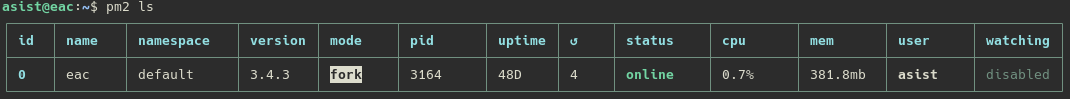
\includegraphics[width=\textwidth,keepaspectratio]{ch5/assets/pm2ls.png}
\caption[PM2 Managed Application List]{PM2 Managed Application List}
\label{fig:pm2}
\end{figure}

The Figure~\ref{fig:pm2} show the list of managed application and some of their details.
EAC is the name given to the Web Application and in the PM2 configuration.
The figure also shows that the application was up for the last 48 days, and that it was automatically restarted 4 times.

In regards to the Explanation API, it was created a Systemd service.
Systemd is a initialization system and service manager native to many Linux distributions such as Ubuntu.

\begin{center}
\begin{minipage}{0.95\linewidth}
\lstinputlisting [caption=Explanation Systemd Service.,
label=lst:explanation-service]
{ch5/assets/explanation.service}
\end{minipage}
\end{center}

In the Listing~\ref{lst:explanation-service} is shown the configuration required to create the service for the Explanation API.
With this service Systemd will manage the API, and will automatically restart it if goes down.

To allow both the Web Application and the Explanation API to be accessible through HTTP it was required to set up a reverse proxy using nginx\footnote{https://nginx.org/en/}.
A reverse proxy is an server sided intermediary server that forwards a user request to the available web servers.

\begin{center}
\begin{minipage}{0.95\linewidth}
\lstinputlisting [caption=Reverse Proxy Configuration.,
label=lst:reverse-proxy]
{ch5/assets/reverse-proxy.conf}
\end{minipage}
\end{center}

As shown in the Listing~\ref{lst:reverse-proxy}, the requests made to the "search" endpoint are forward to the Explanation API while the requests to the base endpoint are forward to the Web Application.

In order to protect the integrity and improve the security of this application the HTTPS protocol was enable in the reverse proxy server.
This was accomplish by using Certbot\footnote{https://certbot.eff.org/} which automatically enables HTTPS in a server running in the HTTP port by deploying Let's Encrypt\footnote{https://letsencrypt.org/} certificates.

\begin{center}
\begin{minipage}{0.95\linewidth}
\lstinputlisting [caption=Reverse Proxy Configuration after Certbot.,
label=lst:reverse-proxy-certbot]
{ch5/assets/reverse-proxy-https.conf}
\end{minipage}
\end{center}

The Listing~\ref{lst:reverse-proxy-certbot} shows an excerpt of the changes made by Cerbot to enable the HTTPS protocol.

\section{Design Changes}

This section will present how the original design changed during the implementation.
The integration with the avatar API and Database was not possible to be implemented, this had a great impact on how the solution ended up being implemented.
Without this two components, the "US03: Display sign language translation" was able to be implemented.

The developed \gls{LGP} formula also depended on the Avatar Database to access the sign data, this was able to still be implemented by using a local database.

The design of the "US04: Change language" had no alteration made during the implemented thus it wont be featured in this section.

\subsection{Logic view}

The changes made to the component diagram presented in Chapter~\ref{chap:Chapter4} are shown in the following diagram.

\begin{figure}[H]
\centering
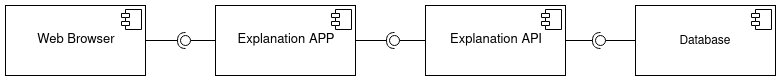
\includegraphics[width=\textwidth,keepaspectratio]{ch5/assets/component_diagram_Implement.png}
\caption[Component Diagram Implementation]{Component Diagram Implementation}
\label{fig:componentImp}
\end{figure}

Shown in Figure~\ref{fig:componentImp} is the component diagram of the solution implemented.
Without the avatar components, there was still a need for a database since the \gls{LGP} formula required sign data to perform the calculation of the readability of each explanation, and this score was a key factor.
This database was seeded with the sign data from the Portuguese table of the Avatar Database.

\subsection{Use cases}

In this section the implemented use cases are presented to better understand the changes made and how they impacted the final solution.

\subsubsection{US01: Find explanation}

\begin{figure}[H]
\centering
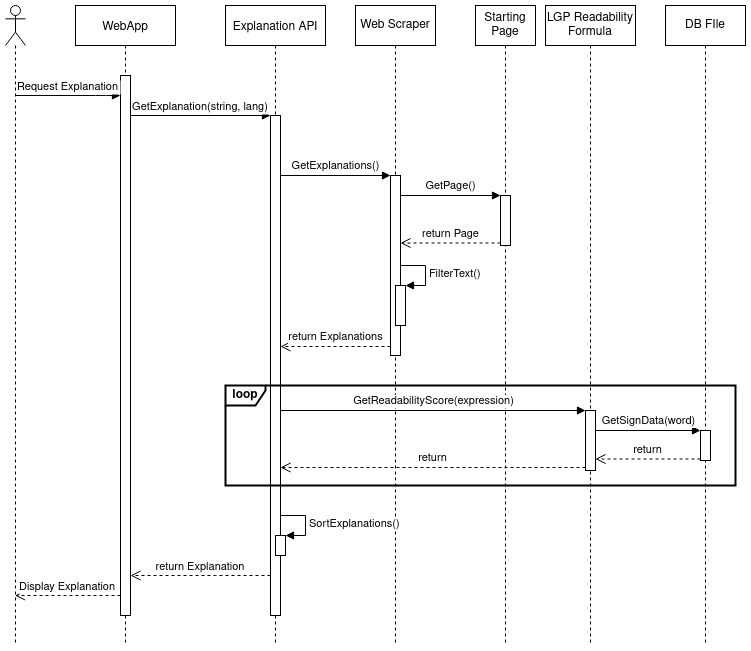
\includegraphics[scale=0.45]{ch5/assets/US01_SD_Implement_Ap1.png}
\caption[Sequence Diagram US01 First Approach]{Sequence Diagram - US01 First Approach}
\label{fig:uc01Imp1}
\end{figure}

In the sequence diagram of Figure~\ref{fig:uc01Imp1} is shown the first approach to obtain an explained previously explained.
This is very different from the diagram presented in the previous chapter since it only resorts to web scrapping to generate explanations.
Also, instead of the design verification it will calculate the readability score of each expression.
For this calculation it queries the local Database file instead of querying the Avatar Database like it was initially designed.
This score is used to sort the explanations is a crescent order.

\begin{figure}[H]
\centering
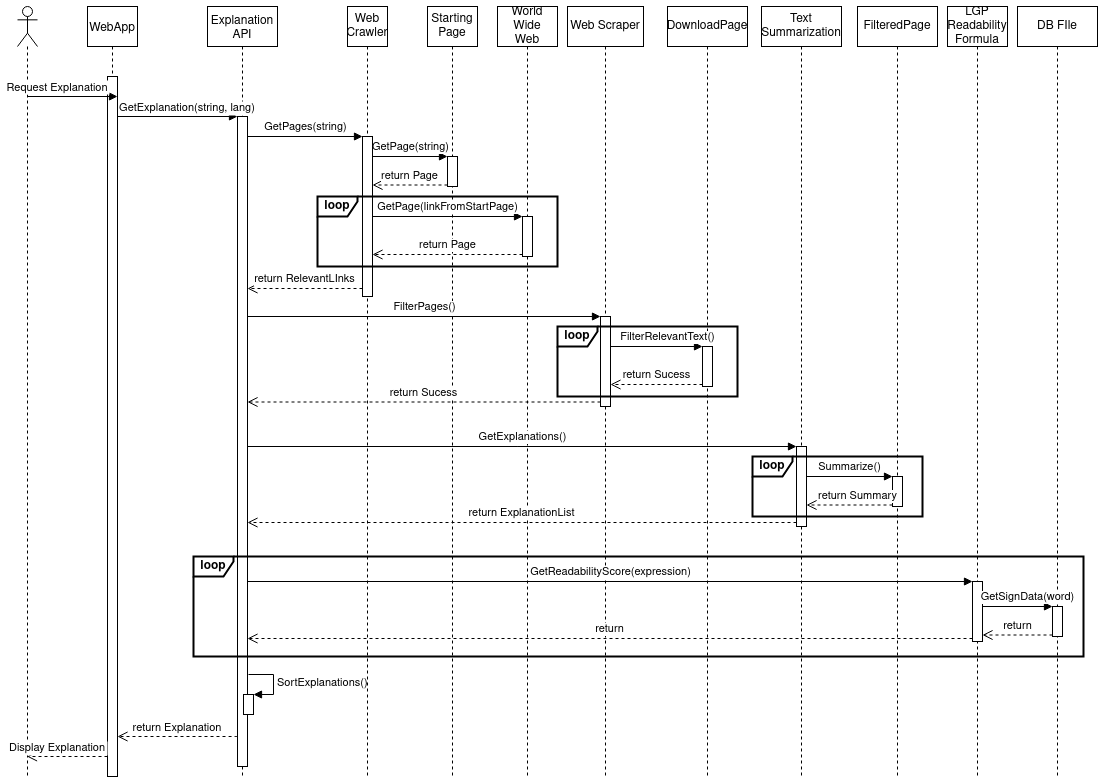
\includegraphics[width=\textwidth,keepaspectratio]{ch5/assets/US01_SD_Implement_Ap2.png}
\caption[Sequence Diagram US01 Second Approach]{Sequence Diagram - US01 Second Approach}
\label{fig:uc01Imp2}
\end{figure}

The sequence diagram displayed in Figure~\ref{fig:uc01Imp2} describes the second approach previously explained.
This is very similar to the diagram presented in Chapter~\ref{chap:Chapter4}.
The main difference is that, like in the first approach, instead of performing a verification to the generated explanation it calculates the readability score and use it to sort the explanations.

\subsubsection{US02: Obtain alternative explanation}

\begin{figure}[H]
\centering
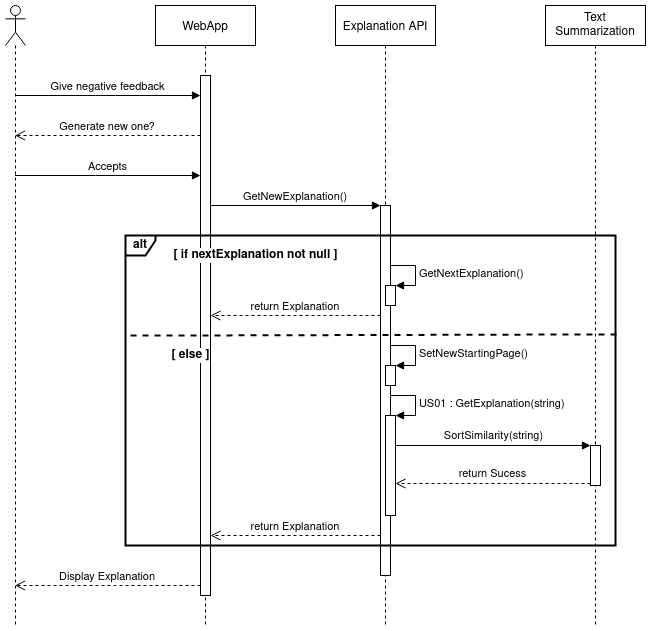
\includegraphics[scale=0.45]{ch5/assets/US02_SD_Implement.png}
\caption[Sequence Diagram Implementation US02]{Sequence Diagram - Implementation US02}
\label{fig:uc02Imp}
\end{figure}

In Figure~\ref{fig:uc02Imp} sequence diagram is shown the implemented process for obtaining a new explanation.
This is also very similar to the diagram presented in Chapter~\ref{chap:Chapter4}.
The main difference is that it requests the text summarization system to sort the new explanation based on similarity as previously mentioned.
No note that to generate new explanation, this will always use the second approach.

\subsection{Deployment view}

The changes made to the deployment diagram presented in Chapter~\ref{chap:Chapter4} are shown in the following diagram.

\begin{figure}[H]
\centering
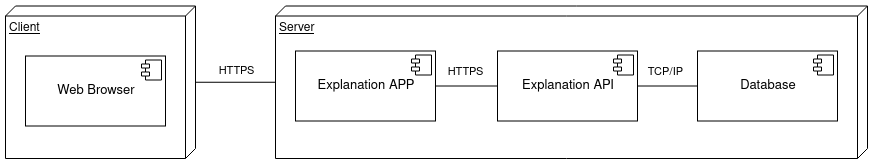
\includegraphics[width=\textwidth,keepaspectratio]{ch5/assets/deployment_diagram_Implement.png}
\caption[Deployment Diagram Implementation]{Deployment Diagram Implementation}
\label{fig:deployImp}
\end{figure}

Shown in Figure~\ref{fig:deployImp} is the deployment diagram of the implemented solution.
As approached throughout this section there is no integration with the Avatar technology, therefor the only change is that there is no interaction with the gilt server.
